\chapter{Multi-Wan Bonding fähigen Treiber für Windows}
\label{chap:Treiber}

\section{Windows Treiber Architektur}
\subsection{Was sind Treiber unter Windows}
Ein Treiber unter Windows ist ein Programm das Windows ermöglicht mit verschiedenen Geräten zu interagieren.\footnote[1]{\cite[Vgl.][]{21}}
\\\\
Die meisten Treiber werden nicht von Windows selber, sondern von Geräte Herstellern programmiert. Geräte Hersteller wissen wie sie mit ihrem Gerät interagieren müssen, um das gewünschte Ergebnis zu erhalten, deswegen schreiben sie die Treiber und nicht die Firma Microsoft. Dadurch ist es Windows möglich so viele verschieden arten von Geräten zu unterstützen.\footnote[2]{Siehe Fußnote 1}
\\\\
Microsoft hat auch Standard Treiber programmiert die mit jeder Windows-Installation beigefügt sind. Diese sind für standardisierte Geräte wie USB Geräte, oder Basis Treiber für CPU und Grafikkarten.\footnote[3]{Siehe Fußnote 1}
\\\\
Es gibt grundsätzlich zwei verschiedene Arten von Treibern. Filter Treiber interagieren selber nicht mit einem Gerät, bearbeiten oder überprüfen aber eine Anfrage und Funktionstreiber kommunizieren dann wirklich mit einem Gerät.\footnote[4]{Siehe Fußnote 1}
\\\\
Normaler weiße gibt es nicht nur einen Treiber, der für ein Gerät zuständig ist. Eine Anfrage läuft über mehrere Filter Treiber bevor es zu einem Funktionstreiber kommt. Diese Abfolge an Treibern nennt man einen Treiber Stack.\footnote[5]{\cite[Vgl.][]{19}}

\newpage

Wenn jetzt eine Applikation mit einem Gerät interagieren will, sendet es zuerst eine Anfrage an Windows. Danach schaut Windows, welcher Treiber Stack für dieses Gerät zuständig, sind und übergibt diese Anfrage in Form eines I/O Request Packets an diesen Treiber Stack. Dieses I/O Request Packet wird dann immer wieder weiterverarbeitet bis es in dem letzten Treiber aus dem Stack ankommt. Wenn dieser dann das I/O Request Packet abgearbeitet hat, übergibt dieser die Daten die ausgewertet wurden wieder an Windows das dann die Daten an die Applikation weitergibt.[siehe Abbildung \ref{windows-driver-stack}]\footnote[1]{\cite[Vgl.][]{19}}\footnote[2]{\cite[Vgl.][]{20}}
\begin{figure}[H]
    \centering
    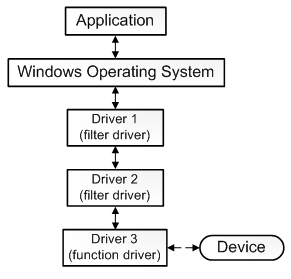
\includegraphics[width=6cm, height=6cm, keepaspectratio]{windows-what-is-a-driver.png}
    \caption[Windows Treiber Stack]{Windows Treiber Stack}[\cite{20}]
    \label{windows-driver-stack} 
\end{figure}
\noindent
\subsection{User vs. Kernel Mode in Windows}
Unter Windows können Programme in zwei verschiedenen Modi laufen. Der erste ist der User Mode in dem alle Applikationen laufen und der zweite in dem die wichtigsten Treiber und Prozesse des Betriebssystem laufen.\footnote[3]{\cite[Vgl.][]{21}}
\\\\
Weil der Kernel Mode in einer geringeren Sicherheitsstufe angesiedelt ist, als der User Mode, hat dieser Hardware mäßig mehr Rechte. Dadurch kann Windows garantieren das Programme die im User Mode laufen nur das machen, was ihnen auch erlaubt ist. \footnote[4]{Siehe Fußnote 3}
\\\\
Programmen im User Mode wird ein virtueller Adressbereich zugeordnet. Dieser Adressbereich hat hauptsächlich zwei Aufgaben. Die erste ist das es Programmen nicht möglich ist Speicher von anderen Programmen anzufordern, einzusehen oder zu bearbeiten. Außerdem hat es den Vorteil das es Windows und das Programm nur lose gekoppelt, dadurch kann das Programm abstürzen ohne das Windows dabei beeinträchtigt wird.\footnote[5]{Siehe Fußnote 3}
\newpage
Programme im Kernel Mode teilen sich wiederum einen Adressbereich mit dem Windows Kernel. Das bedeutet, dass diese Programme die gleichen Rechte haben wie Windows. Dadurch haben diese Programme nicht die Vorteile die sie im User Mode genießen. Es kann also leicht passieren das Programme unabsichtlich auf einen Speicherbereich zugreifen, auf den sie nicht zugreifen wollten und damit entweder ein anderes Programm oder sogar das ganzen System zum Absturz bringen. Aus diesem Grund müssen Treiber die im Kernel Mode laufen extrem gut getestet werden, um sicherzustellen keine Memory Leaks oder Speicherzugriffsverletzung auftreten können. \footnote[1]{\cite[Vgl.][]{21}}

\subsection{I/O request packets}
Ein I/O request packet oder IRP in kurz, sind die Art von Anfragen, die am meisten an Funktionstreiber gerichtet werden. Wenn ein IRP gesendet wird, wird dieser normalerweise von mehreren Treibern im Stack bearbeitet bevor er an seinem Ziel Treiber ankommt.\footnote[2]{\cite[Vgl.][]{23}}
\\\\
Ein IRP besteht hauptsächlich aus einem Buffer und verschiedenen Flags die beschreiben was für eine Operation der Treiber ausführen sollte.\footnote[3]{\cite[Vgl.][]{22}}

\subsection{Geräte Objekte, Geräte Knoten und Geräte Stacks}
In Windows wird jedes Gerät durch einen Geräte Knoten in den Plug and Play (PnP) Geräte Baum abgebildet. Jedes Treiber ist mit einem Geräte Objekt verbunden und diese Geräte Objekte sind dann in einem Stack angeordnet. Jedes Gerät hat wiederum seinen eigenen Geräte Stack.\footnote[4]{\cite[Vgl.][]{24}}
\\\\
Der Geräte Baum wird beim Start von Windows aufgebaut. In Abbildung \ref{windows-plug-and-play-tree} kann man sehen, dass es mehrere Eltern Kind Beziehungen zwischen den einzelnen Geräte Knoten gibt. Die entstehen dadurch das der Root Knoten alle Knoten, die mit ihm Verbunden sind, dazu auffordert alle Knoten die mit diesen Knoten verbunden sind aufzubauen. Dieser Prozess geht so lange, bis alle Knoten aufgebaut wurden. In der Abbildung \ref{windows-plug-and-play-tree} ist also zu sehen, dass der PCI Bus Knoten mehrere andere Knoten aufgebaut hat, wie zum Beispiel den Audio Controller der wiederum ein Audio Device aufgebaut hat. Durch diese Art des Ausbauen und Speichern der Geräte Knoten weiß Windows immer welchen weg IRPs Requests gehen müssen, um an ihrem Ziel Gerät anzukommen.\footnote[5]{Siehe Fußnote 4}
\newpage
\begin{figure}[H]
    \centering
    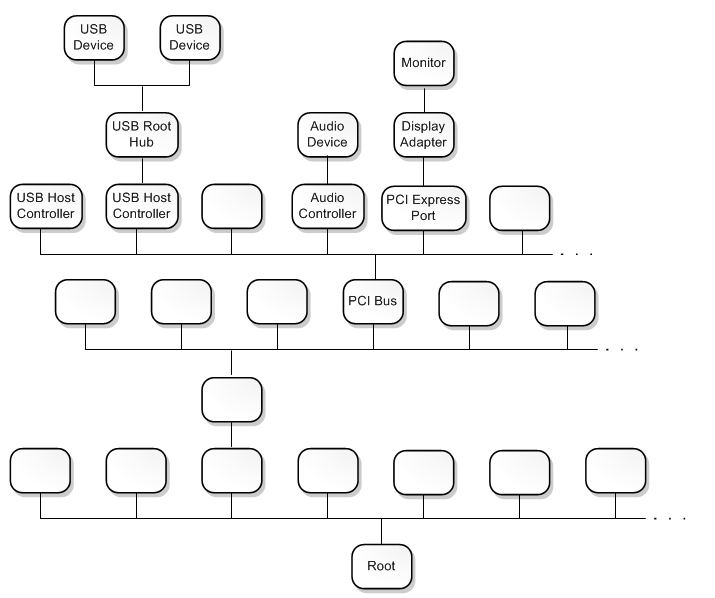
\includegraphics[width=0.9\textwidth]{plug-and-play-device-tree.png}
    \caption[Plug and Play Geräte Baum]{Plug and Play Geräte Baum}[\cite{24}]
    \label{windows-plug-and-play-tree} 
\end{figure}
\noindent
Jeder dieser Geräte Knoten besteht wiederum aus mehreren Geräte Objekten/Treiber Paaren. Diese geordnete Liste an Geräte Objekten und Treiber ergeben an den Geräte Stack für diesen Geräte Knoten. In Abbildung \ref{windows-device-object} kann gesehen werden das der Geräte Knoten PCI Bus einen Geräte Stack hat der aus zwei Geräte Objekt/Treiber Paaren besteht. Das erste Geräte Objekt ist mit dem Treiber Acpi.sys und das zweite mit dem Treiber Pci.sys.\footnote[1]{\cite[Vgl.][]{24}}
\begin{figure}[H]
    \centering
    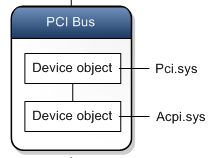
\includegraphics[width=0.4\textwidth]{device-stack.png}
    \caption[Geräte Objekt]{Geräte Objekt}[\cite{24}]
    \label{windows-device-object}
\end{figure}
\noindent

\newpage

\section{Windows Netzwerk Architektur}
Die Netzwerkarchitektur in Windows ist nach den OSI Modell aufgebaut. Das OSI Modell besteht aus sieben Schichten die jeweils eine andere unabhängige Aufgabe. Für unseren Treiber sind jedoch nur die ersten drei Schichten von Bedeutung.\footnote[1]{\cite[Vgl.][]{27}}
\\\\
Die erste Schicht ist die Bitübertragungsschicht, die für das empfangen und versenden von Bits über ein physisches Medium zuständig sind. Physische Medien sind hierbei zum Beispiel Patchkabel, Funknetze und andere. Für diese Schicht sind in Windows die Network Interface Cards (NICs) zuständig.\footnote[2]{Siehe Fußnote 1}
\\\\
Die zweite Schicht ist die Sicherungsschicht, die aus zwei Unterschichten besteht. Die erste Unterschicht ist die MAC Schicht. Diese Schicht hat drei Aufgaben:
\\
\begin{enumerate}
    \item Sie verwaltet den Zugriff auf die Bitübertragungsschicht
    \item Sie überprüft die übertragenen Frames auf Fehler
    \item Sie verwaltet die Adresserkennung von empfangenen Frames
\end{enumerate}
\ \\
Die MAC Unterschicht wird unter Windows von Miniport Treibern\footnote[3]{\cite[Vgl.][]{25}} verwaltet.\footnote[4]{Siehe Fußnote 1}
\\\\
Die zweite Unterschicht ist die LLC Schicht ist für eine fast Fehlerfreie Übertragung von Frames über die Bitübertragungsschicht verantwortlich. Die LLC Unterschicht wird in Windows von Protocol Treiber\footnote[5]{\cite[Vgl.][]{26}} verwaltet.\footnote[6]{Siehe Fußnote 1}
\\\\
Die dritte Schicht ist die Vermittlungsschicht, diese Schicht schaut welchen Physischen Weg das Paket am besten nehmen sollte um in seinem Ziel in seinem Subnetz zu gelangen. Dabei werden auf folgende Faktoren eingerechnet:
\\
\begin{enumerate}
    \item Bedingungen des Netzwerks
    \item Einstellungen vom Priority of Service
    \item Andere Faktoren wie zum Beispiel: Einträge im IP Routing Table, Frame Fragmentierung, …
\end{enumerate}
\ \\
Diese Schicht wird wie die LLC Schicht in Windows von einem Protocol Treiber verwaltet.\footnote[7]{Siehe Fußnote 1}
\\\\
Die Dritte Schicht ist auch die Schicht auf der Wintun arbeitet. Wintun ist unser Treiber der für das Sammeln von IP Paketen und das wieder Einspeisen von Paketen in Windows zuständig ist.\footnote[8]{Siehe Fußnote 1}

\newpage

Wintun\footnote[1]{\cite[Vgl.][]{1}} ist ein TUN Gerät, das bedeutet nur, dass es auf der OSI Schicht 3 arbeitet. Wir hätten auch die Option ein TAP Gerät\footnote[1]{\cite[Vgl.][]{28}} zu verwenden, diese Geräte agieren auf der OSI Schicht 2. Wir haben uns aber gegen ein TAP Gerät entschieden, weil wir in unseren begrenzten Zeit nicht die Ressourcen hatten, das nötige Fachwissen, dass für das Verwenden eines TAP Geräts notwendig ist, aufzubauen.

\section{Architektur des Multi-Wan Bonding fähigen Windows Treibers}
\subsection{Design}
\subsubsection{Anforderungen}

Unser Multi-Wan Bonding Treiber ist dafür verantwortlich Pakete aus Windows zu dem Server zu senden. Dabei müssen 3 Probleme gelöst werden:
\\
\begin{enumerate}
    \item Sammeln von IP Paketen aus Windows
    \item Verteilen von IP Paketen an Programme
    \item Kommunikation zwischen Treiber und Server
\end{enumerate}
\ \\
Außerdem müssen gewisse Standards von Performance, Stabilität und Ressourcenintensität gehalten werden. Dabei haben wir versucht folgende Metriken einzuhalten:
\\
\begin{enumerate}
    \item Maximale prozentuale CPU Auslastung von 5 \%, bei einer 100 Mbit/s Übertragungsrate auf einem AMD Ryzen 7 3700X
    \item Maximaler Speicherverbrauch von 300 Megabyte bei Verwendung von 2 übertragenden Netzwerkadaptern über eine Dauer von 30 Minuten.
    \item Wenn es zum Absturz des Treibers kommen sollte, darf das Betriebssystem nicht mit abstürzen.
    \item Der Treiber sollte weiter funktionieren, auch wenn während des Betriebs ein Netzwerkadapter ausfällt.
\end{enumerate}
\ \\
Zur Bedienungsfreundlichkeit wird ein Command Line Interface (CLI)  zur Verfügung gestellt mit welcher folgende Operationen ermöglicht werden:
\\
\begin{enumerate}
    \item Konfigurieren des Treibers über JSON, Key-Value Dateien oder über die Konsole
    \item Starten und Stoppen der Kommunikation des Treibers mit dem Server
    \item Stoppen und Starten des Treibers
    \item Ausgabe von derzeitigen Einstellungen
\end{enumerate}
\ \\
Die CLI soll über eine lokale TCP Verbindung mit dem Treiber kommunizieren damit sichergestellt werden kann das andere Komponenten leicht eingebunden werden können.

\newpage

\subsubsection{Sammeln von IP Paketen in Windows}
Damit Pakete an den Server versendet werden können, müssen wir dafür sorgen, dass Pakete die von verschiedenen Programmen in Windows verschickt werden durch unseren Treiber leiten. Um Pakete entgegennehmen zu können muss ein virtueller Netzwerkadapter erstellt werden. Dazu verwenden wir den Netzwerktreiber Wintun[1]. Dieser kann performant Pakete empfangen und versenden.
\\\\
Wintun kann jetzt zwar Pakete empfangen. Windows weiß aber noch nicht das es Pakete in den virtuellen Netzwerkadapter umleiten muss. Dafür muss eine statische IP Route im Windows internen IP Routing Table\footnote[1]{\cite[Vgl.][]{2}} eingetragen werden.
\\\\
Nach diesen 2 Schritten werden von Programmen gesendete Pakete, von Windows mithilfe  der Informationen im IP Routing Table, an den Wintun Adapter gesendet und dort durch unseren Treiber verarbeitet. (Für Details siehe Abbildung \ref{driver-collect-packets})
\\\\
\begin{figure}[H]
    \centering
    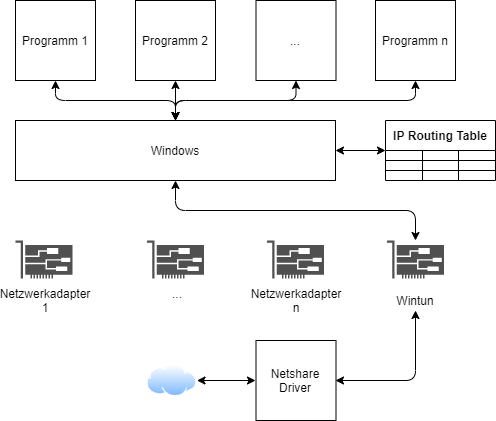
\includegraphics[width=0.8\textwidth]{diagramm_sammel_von_ip_paketen.png}
    \caption[Sammeln von IP Paketen]{Sammeln von IP Paketen}
    \label{driver-collect-packets}
\end{figure}
\noindent

\newpage

\subsubsection{Kommunikation zwischen Multi-Wan Bonding Treiber und Multi-Wan Bonding Server}
Der Treiber kann jetzt Pakete von Windows erhalten und muss diese an den Server schicken. Hierzu war die erste Entscheidung, die wir fällen mussten, auf welche Art wir die Pakete an den Server schicken. Dafür hatten wir zwei Möglichkeiten. Wir verwenden Wintun zum Senden und Empfangen der Pakete vom Server oder wir erstellen einen Socket und lassen über diesen die Kommunikation mit dem Server laufen.
\\\\
Wenn, wir Wintun verwenden haben wir den Vorteil das wir keine weitere externe Bibliothek benutzen müssen und eine höhere Performance haben, weil wir Pakete von OSI Schicht 3 versenden und uns dadurch eine Schicht beim Senden sparen.
\\\\
Der Grund warum wir uns aber dazu entschieden haben Sockets zu nutzen ist der Programmieraufwand. Wir haben zwar bei Wintun eine Performance Steigerung jedoch würde es auch bedeuten, dass wir uns mit dem Aufbau der einzelnen IP Pakete beschäftigen müssen. Was alleine akzeptabel wäre, wenn wir uns nicht auch noch um die Firewalls kümmern müssten. Dadurch, dass Firewalls weiter oben im OSI Modell angelegt sind als unser TUN Gerät\footnote[1]{\cite[Vgl.][]{8}}, müssen wir beim Empfangen von Paketen sicherstellen, das die Firewall diese nicht wegwirft. Das heißt, wir müssen Windows mitteilen, dass wir einen gewissen Port benutzen und Pakete von einer gewissen IP-Adresse erwarten. Aus diesen beiden Gründen und durch unseren bestehenden Zeitdruck haben wir uns dazu entschieden eine Socket Bibliothek zu verwenden.
\\\\
Für die Socket Bibliothek haben wir uns dann für die Windows Sockets 2 API entschieden, weil diese von Microsoft für das Performante verwenden von Sockets unter Windows entwickelt wurde. Außerdem haben wir den Vorteil das wir die Bibliothek nicht selber verwalten müssen, weil diese automatisch von Windows aktualisiert wird.

\subsubsection{Pakete aus dem Multi-Wan Bonding Treiber auf andere Programme des Betriebssystems aufteilen.}
Nachdem wir jetzt Pakete einsammeln können, diese dann an den Server schicken und empfangen können, müssen wir uns nur mehr sicherstellen, dass wir die Pakete aus unserem Treiber wieder an die Programme verteilen können, zu denen sie gehören.
\\\\
Hierfür machen wir uns wieder Wintun zu nutzen, indem wir die Pakete, die wir bekommen haben, nehmen und einfach über unser Wintun Gerät senden. Windows erkennt dann, dass das Paket an sich selbst gerichtet ist und verarbeitet es als wäre es von einem normalen Netzwerk Adapter gekommen. Durch diese Art der Aufteilung lagern wir den meisten Programmieraufwand an Windows aus und können auch für eine hohe Performance garantieren.
\\\\
Fügt man nun alle 3 Überlegungen zusammen, kommt man auf Folgendes. (Für Details siehe Abbildung \ref{driver-full-architecture})
\begin{figure}[H]
    \centering
    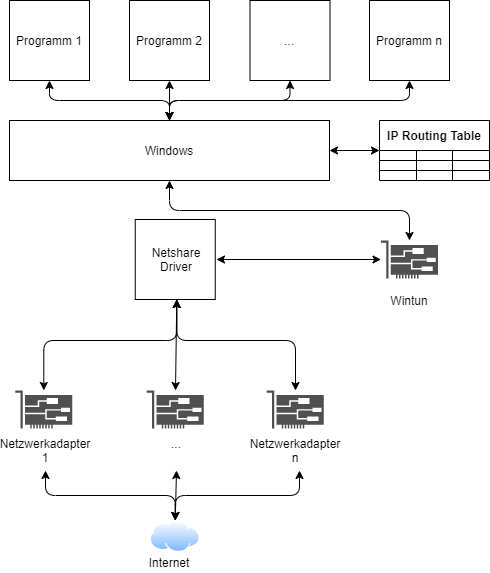
\includegraphics[width=0.8\textwidth]{kommunikation_mit_internet.png}
    \caption[Vollständige Mulit-Wan Bonding Treiber Architektur]{Vollständige Mulit-Wan Bonding Treiber Architektur}
    \label{driver-full-architecture}
\end{figure}
\noindent

\newpage
\subsection{Implementierung}
\subsubsection{IP Pakete Life Cylce}
\paragraph{Erstellen des Eintrags in die IP Routing Tabelle}
\ \\\\
Um IP Pakete umleiten zu können müssen wir Einträge in den IP Routing Table von Windows einfügen. Wie die Codebase des Multi-Wan Bonding Treibers noch nicht ausgereift genug war, haben wir diese Einträge über die Konsole mithilfe des \textbf{route} Befehls eingefügt. Um Pakete in unser Virtual Network Interface Card (VNIC) umleiten zu können müssen wir eine \textbf{default route} erstellen. Als Gateway stellen wir dann die IP-Adresse der VNIC des Multi-Wan Bonding Servers und als Schnittstelle wählen wir die IP-Adresse der VNIC von unserem Multi-Wan Bonding Treiber. Als Metrik haben wir die kleinste Metrik gewählt, die über den route Befehl erstellt werden kann. Dadurch erhalten wir einen Eintrag, der ungefähr so ausschaut:
\\
\begin{center}
    \begin{tabular}{| c | c | c | c | c |}
        \hline
        Netzwerkziel & Netzwerkmaske & Gateway & Schnittstelle & Metrik \\
        \hline
        0.0.0.0 & 0.0.0.0 & 10.0.0.1 & 10.0.0.2 & 7 \\
        \hline
    \end{tabular}
\end{center}
\ \\
Wobei \textit{10.0.0.1} die IP-Adresse des VNICs des Mulit-Wan Bonding Servers und \textit{10.0.0.2} die IP-Adresse des VNCIs unseres Multi-Wan Bonding Treibers ist.
\\\\
Später in der Entwicklung haben wir aber eine programmatische Lösung gebraucht, weil wir nicht davon ausgehen können, dass alle Endnutzer genügend technische Kenntnisse haben, um die Route selber einzustellen. Deswegen benutzen wir Funktionen aus der \textbf{iphlpapi.h}\footnote[1]{\cite[Vgl.][]{6}} Bibliothek. Diese stellt Funktionen zum auslesen und bearbeiten des IP Routing Tables zur Verfügung.
\\\\
Bevor wir eine Verbindung mit dem Server aufbauen lesen wir also den IP Routing Table aus und speichern alle derzeitigen Standard Gateways zwischen und löschen diese danach aus der Tabelle. Nachdem jetzt keine Standardgateways existieren, haben wir das Problem, dass die IP Pakete, die wir zu unserem Server senden wollen, nicht mehr wissen wohin sie weitergeleitet werden sollen. Das heißt, dass alle unsere Pakete nicht zu dem Router weitergeleitet werden. Dadurch kommen diese IP Pakete nicht mehr bei unserem Multi-Wan Bonding Server an. Um dies zu verhindern, erstellen wir neue Einträge, die als Netzwerkziel die IP unseres Servers haben und als Gateway stellen wir die IP-Adresse des VNICs des Multi-Wan Bonding Servers ein. Dadurch stellen wir sicher, dass die Pakete die von unserem Multi-Wan Bonding Treiber verschickt werden, einen Weg finden wie sie über den Router zu unserem Server kommen. Nachdem wir diese Einträge eingefügt haben, erstellen wir einen neuen Eintrag der als Netzwerkziel und als Netzmaske die Standardroute repräsentieren und mit dem Gateway als die IP-Adresse die wir unserer Wintun VNIC zugewiesen haben. Dadurch werden alle Pakete die nicht von einer Route mit einer niedrigeren Metrik oder einer Route die eine höhere Genauigkeit bei dem Netzwerkziel oder Netzwerkmaske aufweist von dieser Route an unsere VNIC weitergeleitet.
\\\\
Wenn die Verbindung wieder abgebaut werden soll, löschen wir die von uns erstellten Einträge wieder, lesen das zwischengespeicherte Standardgateway wieder aus und fügen es in den IP Routing Table ein.
\\\\
Um sicherzustellen das in dem Fall, dass das Programm unerwartet abstürzt, das alte Standardgateway wieder hergestellt werden kann, speichern wir dieses in einer Datei. Diese wird beim Start des Programms ausgelesen und wenn wir erkennen das kein Standardgateway gesetzt ist, stellen wir dieses mit den Informationen aus der Datei wieder her. Um zu verhindern, dass das Standardgateway neu gesetzt wird, obwohl kein Absturz geschehen ist, wird die Datei nach einem erfolgreichen Verbindungsaufbau wieder gelöscht.

\paragraph{Sammeln von Paketen aus Windows}
\ \\\\
Nachdem jetzt sichergestellt wurde, dass alle IP-Pakete, die nicht an das interne Netzwerk oder unseren Server gerichtet sind, an unser VNIC gesendet werden. Müssen wir diese auslesen und zur Weiterverarbeitung zwischenspeichern.
\\\\
Hierzu erstellen wir, falls noch keiner Vorhanden ist, einen virtuellen Wintun Netzwerkadapter. Dieser Netzwerkadapter spiegelt ein TUN Treiber wider, das bedeutet, dass er OSI Layer 3 Pakete weiterverarbeitet. Der Treiber läuft im Kernel Mode\footnote[1]{\cite[Vgl.][]{12}} verarbeitet aber Pakete selber nicht, sondern speichert diese in einem Ringpuffer zwischen\footnote[2]{\cite[Vgl.][]{11}} wo sie von einem sich im Users Mode befindenden Programm weiterverarbeitet werden können. Das hat den großen Vorteil das wir keinen Low Level Windows Code schreiben müssen, wir können davon ausgehen, dass der Treiber stabil läuft und die Integrität des Betriebssystems nicht negativ beeinflusst. Jedoch hat es den Nachteil das der Code, der für das Verarbeiten von IP Paketen zuständig ist, im User Mode läuft, welcher wesentlich langsamer ist als der Kernel Mode. Weil Programme die im User Mode laufen immer wieder auf Funktionen zugreifen müssen die nur im Kernel Mode ausgeführt werden können, müssen diese dann einen Ressourcen aufwendigen Context Switch durchführen\footnote[3]{\cite[Vgl.][]{13}}.
\\\\
Nachdem wir sichergestellt haben, dass es unseren Netzwerkadapter gibt versuchen wir einen Handle auf ihn zu bekommen. In Windows repräsentiert ein Handle eine Ressource auf das ein Programm zugreifen will\footnote[4]{\cite[Vgl.][]{14}}. Das heißt durch Handles hat Windows einen Weg sicherzustellen das zum Beispiel auf Dateien nicht zweimal schreibend zugegriffen werden kann. Wir fordern also einen Handle für unseren Netzwerkadapter an um Operationen an ihm durchführen zu können.
\\\\
Mit dem Adapter Handle, den wir angefordert haben, können wir diesen nun einstellen so wie wir ihn benötigen. Wir stellen also die IP-Adresse, die uns zugewiesen wurde und die dazugehörigen Subnet Bits ein. Danach ist der Netzwerkadapter fertig eingestellt und könnte theoretisch Daten empfangen.
\\\\
Der Netzwerkadapter ist aber noch nicht “eingeschalten” dazu müssen wir eine Session erstellen. In dieser Session können wir einstellen wie groß die Ringpuffer im Treiber sind. Wir haben uns bei der Größe für die maximal von Wintun zugelassene Größe von 64 Mebibyte entschieden. Mithilfe dieser Session können wir, dann anfangen die Pakete, die unser Netzwerkadapter empfangen hat, zu übernehmen und diese weiterzuverarbeiten.

\newpage

\paragraph{Weiterverarbeiten von Paketen}
\ \\\\
Wir können jetzt Pakete von unseren Netzwerkadapter empfangen und diese dann an unser Programm übertragen. Jetzt müssen wir das Paket zwischenspeichern und weiterverarbeiten. Dabei sind wir auf zwei verschiedene Lösungswege gestoßen.
\\\\
Der erste Weg ist das Sammeln und Versenden von IP Paketen auf dem gleichen Thread. Hierbei würde ein IP Paket, das derweil noch im Wintun internen Puffer gespeichert ist, aus diesem in den Multi-Wan Bonding Treiber geladen werden. Nachdem das IP Paket erfolgreich geladen wurde, wird es wiederum in den Puffer eines Sockets geladen und zum Multi-Wan Bonding Server geschickt. 
\\\\
\begin{figure}[H]
    \centering
    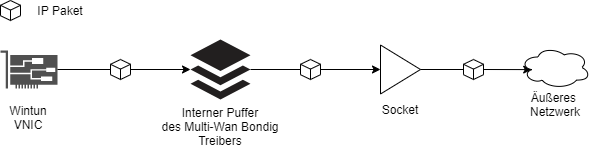
\includegraphics[width=0.9\textwidth]{Verarbeiten_von_IP_Paketen_in_einem_Thread}
    \caption[Verarbeiten von IP Paketen in einem Thread]{Verarbeiten von IP Paketen in einem Thread}
    \label{driver-process-pakets-one-thread}
\end{figure}
\noindent
Das Problem bei diesem Ansatz ist jedoch, dass wir in diesem Fall die Wintun Session an einen Socket binden. Dadurch ist es nicht möglich mehrere Sockets zu erstellen, wodurch es uns nur schwer oder überhaupt nicht möglich ist IP Pakete über mehrere NICs zu versenden. 
\\\\
Die zweite Lösung, die wir auch jetzt noch verwenden ist ähnlich aufgebaut, löst aber das Problem der ersten Lösung. Bei diesem Ansatz wird jeder Socket sowie die Wintun Session zum sammeln von IP Paketen in einem eigenem Thread angesiedelt. Der interne Puffer wird dann in Form einer Thread sicheren Queue implementiert. (Für Details siehe Abbildung \ref{driver-process-pakets-many-threads})

\newpage

\begin{figure}[H]
    \centering
    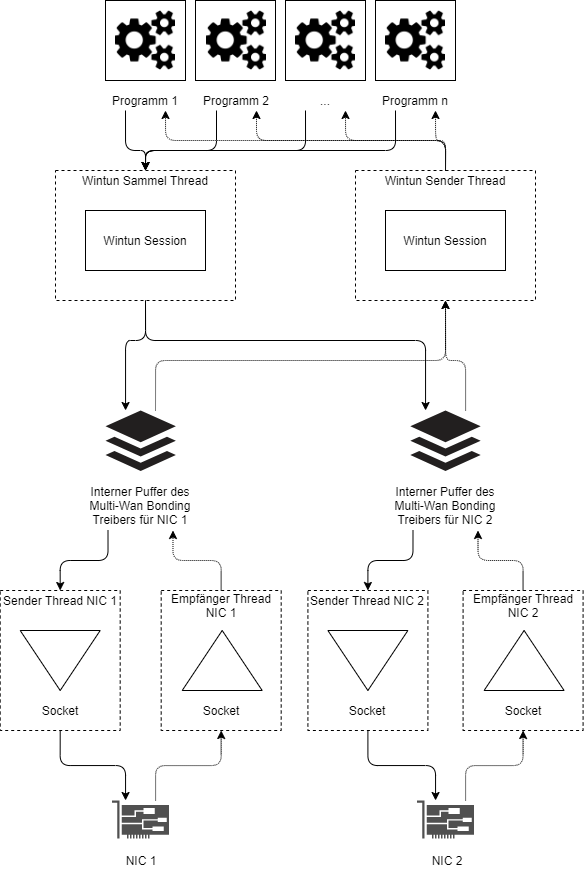
\includegraphics[width=1\textwidth]{verarbeiten_von_ip_paketen_in_mehreren_thread.png}
    \caption[Verarbeiten von IP Paketen in mehreren Threads]{Verarbeiten von IP Paketen in mehreren Threads}
    \label{driver-process-pakets-many-threads}
\end{figure}
\noindent

Wie wir jetzt in Abbildung \ref{driver-process-pakets-many-threads} sehen können erstellen wir für jede NIC die wir verwenden wollen einen internen Puffer.
\\\\
Dieser Puffer besteht aus 2 Thread sicheren Queues. Eine dieser Queues ist für das empfangen und eine für das Versenden von IP Paketen zuständig. Diese Queues sind darauf optimiert mehrere IP Pakete gleichzeitig auszugeben. Das heißt, dass nur 1 IP Pakete gleichzeitig eingefügt werden kann. Aus dem Grund das diese Queues Thread sicher implementiert werden müssen, ist es nicht möglich gleichzeitig IP Pakete auszulesen und einzulagern. Beim Herausnehmen der IP Pakete aus der Queue ist es möglich so viele IP Pakete wie man will gleichzeitig auszulesen. Dadurch können wir sicherstellen, dass die internen Puffer immer schneller entladen werden als sie befüllt werden. Das resultiert dann in einer niedrigeren Verarbeitungszeit und in einer niedrigen Latenz.
\\\\
Um IP Pakete an die Multi-WAN Bonding fähigen Server senden zu können müssen die IP Pakete von dem Wintun Sammel Thread über einen internen Puffer in einen Sender Thread gelangen. 
\\\\
Wenn wir ein IP Paket von unserem Multi-Wan Bonding fähigen Server erhalten, muss dann das IP Paket von einem Empfänger Thread, über den internen Puffer, zum Wintun Sender Thread gelangen.

\paragraph{Versenden von IP Paketen an den Multi-WAN Bonding fähigen Server}
\ \\\\

Die Sender Threads warten so lange, bis in dem internen Puffer des Treibers, der für die NIC zuständig ist, der mit dem Thread verbunden ist, mindestens 1 IP Paket enthalten ist. Solange keine IP Pakete in dem internen Puffer vorliegen schläft der Thread, dadurch erreichen wir das der Thread in dieser Zeit nur extrem wenig Prozessor Ressourcen benötigt.
\\\\
Wenn in dem internen Puffer dann IP Pakete vorliegen erwacht der Thread wieder und versendet alle IP Pakete, die er aus dem internen Puffer bekommen hat. Hierzu werden die IP Pakete dann in einen Puffer eines Sockets kopiert um von dort weiter gesendet werden zu können. 
\\\\
Dieser Socket darf jedoch nur die IP Pakete über eine bestimmte NIC versenden. Um dies zu erreichen, müssen wir den Socket an eine NIC binden. Nachdem ein Socket an eine NIC gebunden wird, werden alle IP Pakete die dieser Socket aussendet über diese NIC versendet. Wenn wir dies nicht machen würden, würde Windows versuchen die am besten geeignete Route für dieses IP Paket über den IP Routing Table zu finden.

\paragraph{Empfangen von IP Paketen vom Multi-WAN Bonding fähigen Server}
\ \\\\
Das Empfangen von IP Paketen vom Multi-Wan Bonding fähigen Server ist ähnlich aufgebaut wie das versenden. Hier gibt es auch jeweils einen Thread, der für eine NIC zuständig ist. Das heißt, dass auch hier der Socket an eine NIC gebunden wird.

\newpage

Der Thread schläft auch hier so lange keine Pakete vom Multi-Wan Bonding Server eintreffen. Dieses Verhalten erreichen wir hier jedoch über ein \textbf{select} Befehl. Der \textbf{select} Befehl wartet so lange bis in dem Socket, den wir ihm zur Verfügung stellen, ein IP Paket in, seinem internen Puffer, bereit ist gelesen zu werden\footnote[1]{\cite[Vgl.][]{18}}. 
\\\\
Nachdem der Thread wieder aufgewacht ist, kopiert dieser alle IP Pakete aus dem Socket in dem ihm zugeordneten internen Puffer. Wenn keine IP Pakete mehr aus dem Socket ausgelesen werden können, schläft der Thread wieder ein und wartet auf neue IP Pakete.

\paragraph{Error Handling}
\ \\\\
Aus dem Grund das wir großen Zeitdruck hatten, hatten wir nicht die Möglichkeit gutes Error Handling in den Multi-Wan Bonding fähigen Treiber einzubauen. Deswegen werde ich hier darüber schreiben, was ich vorhatte in den Treiber einzubauen.
\\\\
Erstens würde alle Sender und Empfänger Threads überwacht werden. Wenn einer der Threads abstürzt soll geprüft werden, ob dieser Thread abgestürzt ist, weil der Socket in diesem Thread geschlossen wurde. Wenn der Socket in diesem Thread geschlossen wurde, bedeutet das die NIC die mit diesem Socket verbunden ist deaktiviert wurde. Hier würde der Thread also nicht nochmal gestartet werden, weil diese NIC nicht mehr mit einem Netzwerk verbunden ist. Wenn jedoch ein anderer Fehler aufgetreten sein sollte, soll der Thread neu gestartet werden. Wenn ein Thread innerhalb von einer Minute mehr als dreimal wegen eines unbekannten Fehlers neu gestartet werden muss, wird ein Fehler Status für diesen Thread aufgerufen. Der Fehler Status besagt nur das etwas in diesem Thread nicht stimmt und aus diesem Grund diese NIC nicht mehr verwendet werden kann. Das heißt, dass falls der andere Thread, der mit der NIC verbunden ist, noch läuft wird dieser gestoppt. Nachdem wird in einer Datei festgehalten das für diese NIC ein Fehlerzustand aufgerufen wurde. Wenn bei einem kompletten Neustart des Multi-Wan Bonding fähigen Treibers noch einmal ein Fehlerzustand auf der gleichen NIC festgestellt wird, wird diese NIC auf eine Blacklist gesetzt und kann nicht mehr von dem Benutzer verwendet werden.
\\\\
Der Multi-WAN Bonding fähigen Treiber wird außerdem in einen Fehlerzustand versetzt, wenn keine NIC zum Verwenden ausgewählt wurde. Wenn keine NIC zum Verwenden ausgewählt wird, würde der Treiber immer noch alle IP Pakete von Windows einsammeln könnte diese aber nicht mehr an den Multi-Wan Bonding fähigen Server schicken. Deswegen verweigert der Multi-Wan Bonding fähiger Treiber in diesem fall das Aufbauen einer Verbindung mit dem Multi-Wan Bonding fähigen Server, und gibt einen Fehlercode zurück. 

\paragraph{Verhalten bei zu großer Datenübertragung}
\ \\\\
Eine Frage, die wir uns stellen mussten, war wie wollen wir das sich unser Multi-WAN Bonding fähigen Treiber verhaltet, wenn mehr Daten versendet werden als die einzelnen Internetverbindungen bereitstellen können. Nach längerer Überlegung sind wir zu der Entscheidung gekommen, dass wir Pakete wegwerfen ab dem Moment wo der interne Puffer voll wird. Es ist in dieser Situation eigentlich egal, ob wir in unserem Multi-Wan Bonding fähigen Treiber die Pakete wegwerfen oder nicht. Wenn der interne Puffer in einem Socket voll wird, würde dieser auch die eintreffenden IP Pakete wegwerfen. Das bedeutet, dass die IP Pakete sowieso weggeworfen werden würden.
\\\\
In der gegen Situation, wenn zu viele IP Pakete eintreffen, haben wir gar nicht die Möglichkeit etwas an dem Standardverhalten von NICs zu beeinflussen. Wenn der interne Puffer einer NIC voll ist, wirft dieser die neu ankommenden IP Pakete weg, bevor wir diese überhaupt zu Gesicht bekommen würden.
\subsubsection{1}{State Management}
\ \\\\
In unserem Multi-Wan Bonding fähigen Treiber gibt es insgesamt drei verschiedene Klasse die Konfigurationen halten. Die Konfiguration Klasse des höchsten Levels ist die Applikations Konfiguration. Diese Konfiguration ist eine Singleton Klasse und kann in der ganzen Applikation abgerufen werden. Dieses Objekt enthält dann auch die niedrigeren Levels an Konfigurationsobjekten.
\\\\
Das mittlere Level ist das Runtime Konfiguration Objekt dieses enthält Informationen die für alle Sender und Empfänger Threads wichtig sind, wie zum Beispiel: IP-Adresse des Servers, IP-Adresse des Multi-Wan Bonding fähigen Treibers. Diese Konfiguration wird im Start-up Prozess erstellt und an alle Threads verteilt. Diese Konfiguration gibt es auch maximal nur einmal.
\\\\
Das niedrigste Level sind die UDP-Socket Konfigurationsobjekte. Diese Konfiguration Objekte werden auch während dem Start-up Prozess erstellt und enthalten Informationen die für die UDP Sender und Empfänger Threads wichtig sind. Über diese Konfigurationsobjekte ist es außerdem möglich auf das Runtime Konfiguration Objekt zuzugreifen. 
\\\\
Das Runtime Konfiguration Objekt und die UDP-Socket Konfigurationsobjekte werden beide in dem Shutdown Prozess des Treibers gelöscht.
\subsubsection{Konfiguration}
\ \\\\
Das Konfigurieren des Multi-Wan Bonding fähigen Treibers erfolgt über einen in den Treiber eingebauten TCP Server. Dieser Server akzeptiert Verbindungen vom Localhost. Über diese Verbindung kann der Server über drei verschiedene arten konfiguriert werden:
\\
\begin{enumerate}
    \item Über das Versenden von JSON Kommandos
    \item Indem dem Multi-WAN Bonding fähigen Treiber gesagt wird das er eine Key-Value Datei auslesen soll.
    \item Indem dem Multi-Wan Bonding fähigen Treiber gesagt wird das er eine JSON Datei auslesen soll.
\end{enumerate}
\ \\
Wenn der Multi-Wan Bonding fähige Treiber über JSON Kommandos konfiguriert wird, kann jeweils nur eine Einstellung gleichzeitig geändert werden.

\newpage

Wenn der Multi-Wan Bonding fähige Treiber über Dateien konfiguriert wird, muss der Pfad angegeben werden über den diese Dateien gefunden werden können. Nachdem der Multi-Wan Bonding fähige Treiber dann die Datei geöffnet hat überprüft dieser, ob diese Datei die richtige Struktur und Felder hat um eingelesen werden zu können. Wenn ein Attribut fehlt oder wenn ein Attribut zu viel ist, liest der Multi-Wan Bonding fähige Treiber diese Datei nicht ein. Wir haben uns für diese Verhalten entschieden um sicherstellen zu können, dass der Endnutzer weiß welche Attribute ihm zur Verfügung stehen und das er auch sofort eine Fehlermeldung bekommt, wenn er ein Attribut falsch geschrieben hat. Der Endnutzer kommt natürlich auch eine Fehlermeldung, wenn ein Wert eingegeben wird der nicht in die Struktur des Attributes reinpasst. Wenn der Endnutzer zum Beispiel in das Attribut \textbf{serverIP} den Wert \textbf{10.301.12.11} eingibt, bekommt er eine Fehlermeldung in der erklärt wird, dass dies eine ungültige IP-Adresse ist. Wenn in einer einzulesenden Datei ein Fehler aufgetreten ist, werden alle vorher konfigurierte Einstellung wieder hergestellt. 
\\\\
Nachdem der Multi-Wan Bonding fähige Treiber durch eine der drei Arten konfiguriert wurde. Speichert er die neue Konfiguration in einer internen Konfigurationsdatei ab. Diese Konfigurationsdatei ist eine Binärdatei, die nicht von dem Endbenutzer bearbeitet werden sollte. Dadurch, dass diese Datei nicht vom Endnutzer bearbeitet wird können wir davon ausgehen, dass die Daten in der Datei nicht fehlerhaft sind und müssen sie also nicht   überprüfen.
\\\\
Wenn der Multi-Wan Bonding fähige Treiber eine Verbindung mit einem Multi-Wan Bonding fähigen Server aufgebaut hat, werden die Änderungen in der internen Konfigurationsdatei festgehalten sie werden aber nicht sofort angewendet. Erst, wenn die Verbindung abgebaut wird, wird die neue Konfiguration angewendet.
\subsubsection{Logging}
Weil bei niedrigen Log Levels in dem Multi-Wan Bonding fähigen Treiber eine große Anzahl an Daten anfallen haben wir uns dazu entschieden die Logs in mehrere Dateien aufzuteilen.
\\\\
Es gibt drei verschieden Arten von Log Dateien.
\\
\begin{enumerate}
    \item Applikations Log Dateien
    \item Worker Log Dateien
    \item Wintun Log Dateien
\end{enumerate}
\ \\
Die Applikations Log Datei enthält alle Log Einträge, die nicht während einer bestehenden Verbindung zu einem Multi-Wan Bonding fähigen Servers entstehen. In dieser Datei sind zum Beispiel Konfigurationsänderungen enthalten.

\newpage

Worker Log Dateien enthalten alle Logs, die in einem der Worker Threads erstellt werden. Ein Worker Thread kann einer der folgenden sein:
\\
\begin{itemize}
    \item Der Wintun Sammel Thread
    \item Der Wintun Sender Thread
    \item Ein UDP Sender Thread
    \item Ein UDP Empfänger Thread
\end{itemize}
\ \\
Jede dieser Dateien wird in einem eigenen Unterordner gespeichert, weil diese Dateien auf eine maximale Größe von 5 Megabyte eingestellt sind. Wenn eine dieser Dateien mehr als 5 Megabyte an speicher verbrauchen würde, wird eine neue Datei erstellt. Dafür haben wir uns entschieden damit diese Datei in einem Textbearbeitungsprogramm geöffnet werden können, ohne das es zu langen Ladezeit kommt.
\\\\
In den Wintun Log Dateien werden alle wichtigen Events die im Wintun Treiber auftreten festgehalten.